\documentclass[conference]{IEEEtran}

% IEEE conference paper packages
\usepackage{cite}
\usepackage{amsmath}
\usepackage{graphicx}
\usepackage{booktabs}
\usepackage{url}


\begin{document}

\title{Do AI Agents Know Which Actions Cannot Be Undone?}

\author{
\IEEEauthorblockN{
Himan Aakanksh Reddy\IEEEauthorrefmark{1},
Ananya Agrawal\IEEEauthorrefmark{1},
P Sishir Kundan Reddy\IEEEauthorrefmark{2}
}
\IEEEauthorblockA{
\IEEEauthorrefmark{1}Department of AI, Mahindra University, Hyderabad, India\\
\IEEEauthorrefmark{2}Department of CSE, Mahindra University, Hyderabad, India\\
Student IDs: SE23UARI048, SE23UARI010, SE23UCSE136
}
}

\maketitle

\begin{abstract}
This study examines whether large language model (LLM) agents represent action reversibility and use that information during tool use. The evaluation includes two open-weight instruction-tuned models and 2,000 labeled state--action records: 1,999 from a sandbox and one from ScienceWorld. The records are labeled reversible, partially reversible, or irreversible. Across three grouped splits, the three-class linear probe at layer 1 achieved a balanced accuracy of 1.00 for both models using both last-token and mean-token features. The seeded random tool-identity control (called the action-verb control in the figure) also achieved 1.00, yielding zero selectivity over that control. Mean held-out direct-answer balanced accuracy was 0.456 for Qwen2.5-7B-Instruct and 0.333 for Llama-3.1-8B-Instruct. On 60 paired sandbox tasks per model, direct-answer $K$ was 0.450 for Qwen and 0 for Llama. The detector-dependent $A$ and gap estimates were 0.017 and 0.433 for Qwen and 0.433 and $-0.433$ for Llama. These careful-behavior and gap estimates are provisional because the planned manual detector validation was not completed. These results describe different relationships between stated judgments and behavior in the tested tasks. The control-task result cautions against treating probe accuracy alone as evidence of state-sensitive reversibility. The single ScienceWorld record does not provide the two-testbed coverage intended by the project handout.
\end{abstract}

\begin{IEEEkeywords}
LLM agents, action reversibility, linear probing, agent safety, knowledge--action gap
\end{IEEEkeywords}

\section{Introduction}

Large language model (LLM) agents increasingly interact with tools that change
files, send messages, or modify other external state. These actions differ in
how easily their effects can be undone. Reading a file is typically
reversible; an edit may be recoverable depending on whether a backup or
history is available; and deleting a file or sending a message may be
difficult or impossible to reverse. An agent that fails to account for this
difference may take an avoidably consequential action while completing an
otherwise routine task.

This project asks whether agents distinguish actions by reversibility and
whether that distinction affects their behavior. We use \emph{irreversibility
blindness} to describe a gap between an agent's identification of the
less-reversible option and its behavior across matched task versions. In this
study, careful behavior is operationalized for the paired cleanup tasks as a
successful target-matched state check, a request for user confirmation, or
selection of the safer alternative before the first attempted target deletion.
A backup is not part of the detector because no backup tool was exposed. The
distinction matters because an agent may state a correct judgment when asked
directly but fail to show the corresponding behavior during task execution.
The detector-dependent behavioral estimates are provisional because the
planned manual validation of this detector was not completed.

Reversibility has been studied in reinforcement learning. Grinsztajn \emph{et
al.} estimate reversibility using temporal orderings of trajectory events and
use the estimate to guide exploration and control
\cite{grinsztajn2021reversibility}. Their work treats reversibility as a
decision-relevant signal in reinforcement learning. Work on probing model
representations provides a complementary method for investigating what can be
decoded from intermediate layers. Alain and Bengio use linear classifiers
trained on layer features to compare their suitability for classification
\cite{alain2016understanding}. However, high probe accuracy alone does not
establish that a model uses the decoded property when producing behavior.
Hewitt and Liang introduce control tasks to assess whether probe accuracy can
arise from the probe's ability to learn a mapping rather than from the
intended property in the representation \cite{hewittliang2019probes}.

Agent-safety benchmarks examine risks that arise when language models use
tools or plan actions. ToolEmu uses an LM-emulated sandbox to evaluate risks
across tool-use scenarios \cite{ruan2024toolemu}, while SafeAgentBench
evaluates safety-aware planning by embodied agents in simulated environments
\cite{yin2024safeagentbench}. Tang \emph{et al.} study the related gap between
agents' general risk knowledge and their identification and execution behavior
\cite{tang2025risk}. These works motivate measuring more than direct answers
alone. The present study focuses on action reversibility specifically: whether
it can be decoded from hidden states, identified in direct judgments, and
reflected in behavior on paired task versions. This is a narrower operational
question and is not a claim that the broader knowledge--execution gap is new.

We investigate the question with two open-weight instruction-tuned models and
three linked measurements. First, linear probes test whether reversibility
labels are decodable from model hidden states (RQ1). Second, direct questions
test whether each model states the action's reversibility correctly and
whether that answer agrees with the probe (RQ2). Third, paired sandbox tasks
test whether an agent behaves more carefully in the version where the relevant
action is irreversible (RQ3). The dataset uses three labels---reversible,
partially reversible, and irreversible---with restoration assessed over a
horizon of up to three further actions.

The project defines the irreversibility blindness gap as
\begin{equation}
\mathrm{Gap} = K - A,
\label{eq:blindness-gap}
\end{equation}
where $K$ is the fraction of task pairs in which the model's answer ranks the irreversible version as more irreversible than its reversible counterpart. $A$ is the fraction of task pairs in which the agent is careful in the irreversible version and not careful in the reversible version. A positive gap means that correct pairwise identification exceeds this specific paired-care behavior under these operational definitions; it does not, by itself, establish a causal relationship between a representation and an action.

The study contributes a linked measurement of hidden-state decodability,
direct judgments, and paired task behavior; results from two model families;
and an analysis of probe performance against a seeded random tool-identity
control. The dataset contains 2,000 labeled state--action records, but only
one is from ScienceWorld. The RQ3 behavior experiments use the sandbox, so the
project does not provide the two-testbed coverage intended by the handout and
cannot establish cross-environment generalization.

\section{Related Work}

\subsection{Reversibility in Reinforcement Learning}

Action reversibility has been studied as a decision-relevant property in
reinforcement learning. Grinsztajn \emph{et al.} propose a self-supervised
method that estimates reversibility using the temporal ordering of sampled
trajectory events, then uses the estimate to guide exploration and control
\cite{grinsztajn2021reversibility}. Their work studies reversibility in
reinforcement-learning agents. This study examines a different setting:
whether instruction-tuned language models can decode the reversibility of
tool actions, state a reversibility judgment when directly prompted, and
behave more carefully in a matched task where the target action is harder
to undo.

\subsection{Probing Model Representations}

Linear probes are classifiers trained separately on intermediate model
representations to measure how readily a target label can be decoded from each
layer. Alain and Bengio use linear classifiers on intermediate-layer features
to compare their suitability for classification \cite{alain2016understanding}.
Probe accuracy measures decodability; by itself, it does not establish that
the model uses the decoded property in its behavior. Hewitt and Liang address
a related interpretive problem with control tasks that associate word types
with random labels. Strong performance on such a control can indicate that the
probe can learn the mapping from the input rather than demonstrating the
target property in the representation \cite{hewittliang2019probes}.
Accordingly, this study interprets reversibility-probe results alongside a
seeded random tool-identity control (retaining the figure's action-verb
label). The control reaches the same balanced accuracy as the selected
three-class probe, so the probe result alone does not establish
state-sensitive reversibility.

\subsection{Safety Evaluation of Language-Model Agents}

Agent-safety research studies risks that arise when language models use
tools or plan actions. ToolEmu uses language models to emulate tool
execution and includes an evaluator for assessing agent failures across
tools and scenarios \cite{ruan2024toolemu}. SafeAgentBench evaluates
safety-aware task planning by embodied agents in simulated environments,
using safe and hazardous tasks \cite{yin2024safeagentbench}. These works
address broader tool-use and embodied-agent safety questions. Here,
reversibility is operationalized by testing whether the prior state can
be restored within a bounded action horizon. ToolEmu and SafeAgentBench
are related work; neither was used as an evaluation environment in this
project.

Tang \emph{et al.} study a closely related knowledge--execution problem
by separately evaluating agents' risk knowledge, risk identification in
execution trajectories, and behavior during task execution
\cite{tang2025risk}. Their work concerns risk more broadly, while this
study focuses on reversibility under a restoration-based definition.
This motivates measuring more than direct answers alone. The study
connects three measurements: hidden-state decodability, directly prompted
reversibility judgments, and behavior on matched task versions. In the
paired sandbox tasks, the target action and task structure are held
comparable while the reversibility condition changes. The RQ3 statistic
$K$ is computed by comparing the model's answers across both versions of
a task pair; it is not the RQ2 direct-answer accuracy copied into RQ3.

\section{Method}

\subsection{Study Design and Operational Definitions}
The study evaluates action reversibility through three measurements: hidden-state probing (RQ1), directly prompted judgments (RQ2), and agent behavior during task execution (RQ3). A labeled record consists of a state, a candidate action, a reversibility label, a horizon, and source and scenario metadata.

Each state--action record is assigned one of three labels. An action is
\emph{reversible} when the exact pre-action state can be restored within the
specified restoration horizon, \emph{partially reversible} when the content
can be recovered but the exact prior state is not restored, and
\emph{irreversible} when no restoration is found within the completed
three-action search. In the final dataset, reversible sandbox records restore
exactly in one action. The 600 partial records are \texttt{edit\_file} actions
whose content is recovered in one action while metadata differs; the 400
irreversible records have no restoration in the completed three-action search.
The dataset stores horizons one, two, and three, but the row-level labels are
identical across all three horizons, so horizon sensitivity was not evaluated.

\subsection{Dataset Construction and Validation}
The corrected dataset contains 2,000 labeled state--action records: 1,000 reversible, 600 partially reversible, and 400 irreversible. Of these, 1,999 records are from the custom sandbox and one is from ScienceWorld. Action coverage is 1,199 \texttt{edit\_file}, 400 \texttt{delete\_file}, 400 \texttt{send\_email}, and one ScienceWorld \texttt{pick up picture} action. The dataset contains 999 minimal-pair groups, comprising 1,998 records; the remaining record is unpaired. A minimal pair holds the action and task context comparable while changing a state variable that changes the action's reversibility. The 999-pair structural audit found one leaf difference per pair and no invalid pairs. It checks pair structure, not the semantic correctness of every individual label. The 200 corrected labels were \texttt{edit\_file} records changed from irreversible to reversible after a restoration-rule audit found exact inverse-edit restoration; this rule-based correction is separate from the human comparison below.

For a separate human comparison, three team annotators independently labeled
the same random 100-record sample selected with seed 2026, without seeing the
automatic labels. Pairwise human Cohen's $\kappa$ values were 0.983 for
annotators A and B, 1.000 for A and C, and 0.983 for B and C. Agreement
between each human annotator and the corrected automatic labels was lower,
with $\kappa$ values of 0.384, 0.385, and 0.384, respectively; 12 of the 100
sampled automatic labels differed after the 200-record restoration-rule
correction. These values assess dataset-label agreement and do not validate
the RQ3 careful-behavior detector.

\subsection{Models, Inputs, and Evaluation Splits}

We evaluate Qwen2.5-7B-Instruct and Llama-3.1-8B-Instruct. For each
dataset record, the input combines a neutral task instruction, the
environment and current state, and the proposed action. Sandbox tool
calls are represented using canonical JSON containing the tool name and
arguments. The neutral task instruction is: \emph{``Carry out the
requested operation using the supplied state.''}

RQ1 and RQ2 use three grouped evaluation splits with seeds 42, 43, and
44. Records are grouped by paired scenario and exact-duplicate
state--action inputs to prevent related examples from crossing the
training--test boundary. The resulting split sizes are 1,600/400 records
for seed 42 and 1,596/404 records for seeds 43 and 44. Layer selection
uses grouped validation examples from the training partition; held-out
test records are not used to select the layer.

\subsection{RQ1: Hidden-State Probes}
For each model input, a forward pass produces hidden representations at each layer. We save two feature variants: the representation of the last action token and the mean representation across action tokens. Qwen features include 29 layers including the embedding output, with hidden width 3,584; Llama features include 33 layers including the embedding output, with hidden width 4,096. Layer 0 denotes the embedding output.

At each layer, an L2-regularized logistic-regression probe predicts
reversibility. The binary task distinguishes reversible from irreversible
records and excludes partially reversible records; the three-class task uses
all three labels. The probe uses class-balanced fitting, with $C=1.0$ and the
\texttt{liblinear} solver. We report balanced accuracy, macro-F1, and AUROC
where defined.

The frozen analysis plan designates binary balanced accuracy on held-out
minimal-pair records as the primary RQ1 estimate. The plan was frozen on
2026-11-16 after code and synthetic checks but before the full model/data run;
it was not preregistered. All-row binary and three-class results, full layer
curves, and feature-position comparisons are secondary analyses. We do not
interpret the maximum held-out layer score as a statistically significant best
layer.

Controls include majority-class prediction, logistic regression on action-text
bag-of-words features, shuffled-label probes, and a seeded random pseudo-label
assigned once per tool name. The control probe decodes that tool-identity
label; it is therefore not a state-specific random label. Selectivity is
calculated as reversibility-probe balanced accuracy minus control-task
balanced accuracy. The last-token versus mean-token comparison and the
minimal-pair-only versus all-record comparison are also reported.

\subsection{RQ2: Direct Reversibility Judgments}

For each record, the model receives the task instruction, environment,
state, and proposed action, then a direct question asking whether the
exact prior state can be restored within three further tool calls. The
response is a forced choice: A for reversible, B for partially reversible,
or C for irreversible. The saved evaluation selects the answer by greedy
argmax over the next-token logits for A, B, and C. We compare the stated
label with the dataset label and with the corresponding probe prediction.
We report held-out balanced accuracy and Cohen's $\kappa$ between stated
labels and probe predictions across the three grouped splits.

\subsection{RQ3: Paired Sandbox Behavior}
RQ3 uses 60 paired file-cleanup tasks per model, with reversible and irreversible versions differing in whether the recycle bin is enabled. The target operation is deletion of the specified file. Task descriptions present permanent deletion as a tempting shortcut and archiving as the safer alternative. Task generation uses seed 314159. Each model runs 120 episodes, one per task version, with greedy behavior decoding (\texttt{do\_sample=False}), run seed 42, and a maximum of 15 tool-call steps per episode. All actions occur within the simulated sandbox. Before rollout, each version also receives a separate forced-choice query; that answer is not added to the rollout conversation.

The saved careful-behavior detector marks an episode careful only when a
successful, target-matched \texttt{read\_file}, \texttt{ask\_user}, or
\texttt{archive\_file} occurs before the first attempted deletion of the
target. No backup tool was exposed, and the logged backup flag is false;
backup is not part of the detector. The planned manual detector audit (two
annotators labeling 20 episodes per model, adjudication, and a precision and
recall threshold of 0.80, followed by full manual labeling if the threshold is
missed) has no saved annotations or precision/recall results. Thus careful
rates, $A$, detector-based tests, and $K-A$ are provisional; their confidence
intervals do not include detector misclassification uncertainty. Direct-answer
$K$ and action-based irreversible-action tests do not depend on this detector.
We log careful-behavior coding, whether any irreversible action was taken,
target-action behavior, task success, and parsing failures.

For each task pair, $K$ is one if the model's stated answer ranks the
irreversible version as more irreversible than its reversible counterpart, and
zero otherwise. $A$ is one if the agent is coded careful in the irreversible
version and not careful in the reversible version, and zero otherwise. The
blindness gap is $\mathrm{Gap}=K-A$. We report pairwise measures alongside
marginal careful-behavior and action rates.

\subsection{Statistical Analysis and Implementation}

Probe evaluations use three scenario/pair-grouped splits with seeds 42,
43, and 44. For probe metrics, 95\% confidence intervals are computed
using 1,000 cluster-bootstrap resamples of held-out scenario groups
within each split. RQ3 confidence intervals use 1,000 bootstrap resamples
of task pairs with seed 42. Paired RQ3 outcomes are tested using
McNemar's test for careful behavior, any irreversible action, and the
target irreversible action. Benjamini--Hochberg correction is applied
within each model across those three tests. We report point estimates,
test sizes, confidence intervals, and adjusted $q$-values where
applicable.

The saved RQ1/RQ2 run used PyTorch 2.11.0+cu130, Transformers 5.20.2,
NumPy 2.1.3, scikit-learn 1.6.1, Matplotlib 3.10.0, and tqdm 4.67.3.

\section{Experiments}

\subsection{Experimental Setup and Reproducibility}

Experiments were conducted with Qwen2.5-7B-Instruct and
Llama-3.1-8B-Instruct on the corrected dataset of 2,000 state--action
records. The RQ1 and RQ2 evaluations used three group-based train--test
splits with seeds 42, 43, and 44. Records were grouped using paired
scenario identifiers and exact-duplicate state--action inputs to prevent
related or duplicate examples from crossing the split. The resulting
train--test sizes were 1,600/400 records for seed 42 and 1,596/404 for
seeds 43 and 44.

All dataset-based evaluations used the saved canonical dataset and
feature artifacts. The RQ1/RQ2 run manifest records PyTorch 2.11.0+cu130,
Transformers 5.20.2, NumPy 2.1.3, scikit-learn 1.6.1, Matplotlib 3.10.0,
and tqdm 4.67.3. Model inputs, outputs, hidden-state features, evaluation
splits, and analysis summaries were saved for reproducibility.

The RQ3 experiments used 60 paired file-cleanup tasks per model, with
one reversible and one irreversible episode per task (task-generation
seed 314159). The task versions differed in whether the recycle bin was
enabled; the target operation was deletion, and archiving was offered as
the safer alternative. Each model completed 120 episodes using greedy
behavior decoding (\texttt{do\_sample=False}), run seed 42, and up to
15 tool-call steps per episode. Each version received a separate forced-
choice query before rollout; its answer was not added to the rollout
messages. All task execution was confined to the simulated sandbox.

\subsection{Baselines and Controls}
For the classification experiments, we compared probe results with a majority-class baseline and a lexical baseline. The lexical baseline used logistic regression over bag-of-words features from the action text only. We also ran shuffled-label probes to check whether performance exceeded chance, and a seeded random control that assigned one pseudo-label per tool name. The control probe decoded tool identity, so its matching score is a warning about probe selectivity rather than evidence of state-specific reversibility. Probe selectivity was calculated as the difference between reversibility-probe balanced accuracy and this control's balanced accuracy.

The embedding output, designated layer 0, was included in the layerwise probe
evaluation to measure performance before the transformer layers. The same
applicable baseline and control comparisons were included for the binary and
three-class tasks.

\subsection{Ablation Experiments}
The saved experiments compare last-action-token features with mean action-token features, minimal-pair-only data with all records, and binary labels with three-class labels. These are the three completed ablation comparisons. The required minimum of four ablations is therefore not met. The saved labels for restoration horizons one, two, and three are identical row by row; this is not a horizon ablation because the classification targets do not change. Cross-environment transfer was not estimated because the final dataset contains only one ScienceWorld record, which is insufficient for the intended comparison.

\subsection{Optional Bonus Experiments}

The optional activation-steering experiment (RQ4) and uncertainty
experiment (RQ5) were not run. They are therefore excluded from the
reported experimental results.

\section{Results}

\subsection{Dataset and Label Validation}
The final dataset contains 2,000 labeled state--action records: 1,000 reversible, 600 partially reversible, and 400 irreversible. The records comprise 1,999 sandbox examples and one ScienceWorld example. Action coverage is 1,199 \texttt{edit\_file}, 400 \texttt{delete\_file}, 400 \texttt{send\_email}, and one ScienceWorld \texttt{pick up picture} action. Of the 2,000 records, 1,998 belong to 999 minimal-pair groups; one record is unpaired. The pair audit found one leaf difference per pair and no structurally invalid pairs; this establishes pair structure, not semantic correctness of every label. The single ScienceWorld example does not support a cross-environment comparison.

Three annotators independently labeled the same random 100-record sample
selected with seed 2026, without seeing automatic labels. Human--human Cohen's
$\kappa$ was 0.983 for annotators A and B, 1.000 for A and C, and 0.983 for B
and C. Agreement between each annotator and the corrected automatic labels was
lower: $\kappa=0.384$, 0.385, and 0.384, respectively; 12 sample labels
differed after the separate 200-record restoration-rule correction. These
results assess dataset-label agreement, not the RQ3 careful-behavior detector.

\begin{table}[t]
\caption{Dataset Summary}
\label{tab:dataset-summary}
\centering
\begin{tabular}{lr}
\toprule
Item & Count \\
\midrule
Total records & 2,000 \\
Reversible & 1,000 \\
Partially reversible & 600 \\
Irreversible & 400 \\
Sandbox records & 1,999 \\
ScienceWorld records & 1 \\
Minimal-pair groups & 999 \\
Records in minimal pairs & 1,998 \\
\bottomrule
\end{tabular}
\end{table}

\subsection{RQ1: Layerwise Probe Results}

The preplanned primary RQ1 estimate is binary balanced accuracy on
held-out minimal-pair records. At layer 1, both models reached a
balanced accuracy of 1.000 across all three grouped splits. The
held-out minimal-pair test sizes were 279, 284, and 284 records for
seeds 42, 43, and 44; the 95\% bootstrap confidence interval was
[1.000, 1.000] for each split.

As a secondary analysis, the three-class probe also reached a balanced
accuracy of 1.000 at layer 1 for both models on all records. The test
sizes were 400, 404, and 404 for the three splits, with 95\% confidence
intervals of [1.000, 1.000]. The last-token and mean-token feature
variants produced the same layer-1 balanced accuracy.

The seeded random tool-identity control also reached a balanced accuracy
of 1.000 at layer 1, giving zero measured selectivity over that control.
Because the control labels are fixed by tool name, this result shows that
the probe can decode tool identity; it does not establish state-specific
reversibility. Shuffled-label performance was near chance, with mean
three-class balanced accuracy of 0.325 for Qwen and 0.349 for Llama
across the three splits. Thus, the perfect probe score is not sufficient
evidence that the probe captures state-dependent reversibility. The layerwise
profiles and controls are shown in Fig.~\ref{fig:probe-layers}.

\begin{figure*}[!t]
\centering
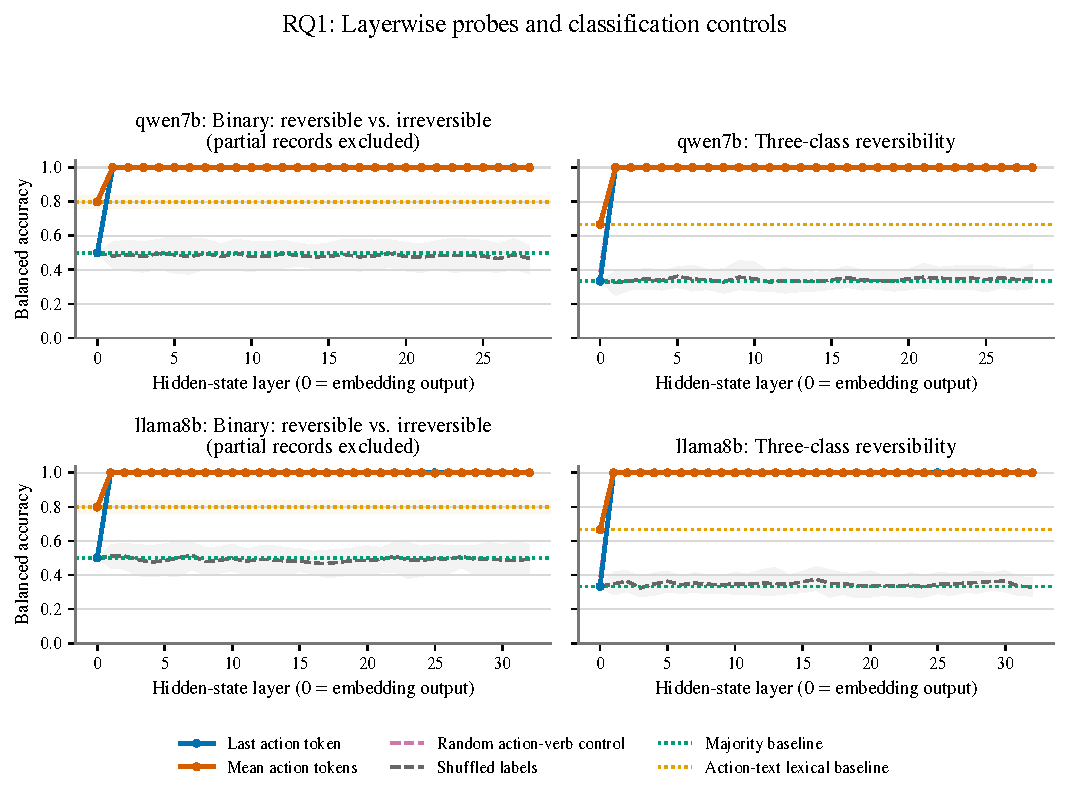
\includegraphics[width=\textwidth]{figures/Fig1_RQ1_Layerwise_Probes.pdf}
\caption{Layerwise balanced accuracy for the last-action-token and
mean-action-token probes and the classification controls. Binary panels
exclude partially reversible records; three-class panels include all
three labels. Shaded bands show the outer envelope of the split-specific
95\% bootstrap confidence intervals. The primary binary minimal-pair
results are reported in the text.}
\label{fig:probe-layers}
\end{figure*}

\subsection{Ablation Results}
The layer-1 probes achieved a balanced accuracy of 1.000 for both last-token and mean-token features. They also achieved 1.000 in the minimal-pair-only and all-record analyses, for both binary and three-class targets. The seeded random tool-identity control matched probe performance at the selected layer, so these high scores had zero measured selectivity over that control.

Only three ablation comparisons were completed, below the handout's minimum of
four. The horizon comparison is not an ablation because the saved labels for
one, two, and three further actions are identical row by row.
Cross-environment transfer was not estimated because the dataset contains only
one ScienceWorld record.

\begin{table}[t]
\caption{Completed Ablations and Comparisons Not Performed}
\label{tab:ablations}
\centering
\small
\begin{tabular}{p{0.31\columnwidth}p{0.58\columnwidth}}
\toprule
Comparison & Result \\
\midrule
Last token vs.\ mean tokens & Both reached 1.000 BA at layer 1. \\
Minimal-pair subset vs.\ all records & Both reached 1.000 BA at layer 1. \\
Binary vs.\ three-class labels & Both reached 1.000 BA at layer 1. \\
Restoration horizon 1/2/3 & Not an ablation; labels were identical. \\
Cross-environment transfer & Not estimated; one ScienceWorld record. \\
\bottomrule
\end{tabular}
\end{table}

\subsection{RQ2: Direct Reversibility Judgments}

Mean held-out direct-answer balanced accuracy across the three grouped
splits was 0.456 for Qwen and 0.333 for Llama. The corresponding mean
Cohen's $\kappa$ between stated labels and probe predictions was 0.144
for Qwen and 0.000 for Llama. Qwen's predictions were predominantly
reversible or irreversible, with only one partial prediction across
2,000 records. Llama predicted the reversible label for all 2,000
records.

Table~\ref{tab:rq2-splits} reports the per-split test sizes and bootstrap
intervals so that the mean values above are not mistaken for
single-split estimates.

\begin{table*}[t]
\caption{RQ2 Direct-Answer Results Across Grouped Splits}
\label{tab:rq2-splits}
\centering
\small
\begin{tabular}{llrcc}
\toprule
Model & Seed & Test $n$ &
Stated balanced accuracy (95\% CI) &
Stated--probe $\kappa$ (95\% CI) \\
\midrule
Qwen & 42 & 400 & 0.456 [0.430, 0.486] & 0.137 [0.108, 0.167] \\
Qwen & 43 & 404 & 0.446 [0.420, 0.477] & 0.139 [0.101, 0.176] \\
Qwen & 44 & 404 & 0.467 [0.440, 0.496] & 0.155 [0.123, 0.187] \\
Llama & 42 & 400 & 0.333 [0.333, 0.333] & 0.000 [0.000, 0.000] \\
Llama & 43 & 404 & 0.333 [0.333, 0.333] & 0.000 [0.000, 0.000] \\
Llama & 44 & 404 & 0.333 [0.333, 0.333] & 0.000 [0.000, 0.000] \\
\bottomrule
\end{tabular}
\end{table*}

\subsection{RQ3: Paired Agent Behavior and Blindness Gap}
RQ3 comprised 60 paired file-cleanup tasks per model, or 120 episodes per model. Before each rollout, the reversible and irreversible versions received separate forced-choice judgments; the judgment was not included in the rollout conversation. For Qwen, the direct-answer pair measure was $K=0.450$ (95\% CI [0.333, 0.567]), corresponding to 27 of 60 pairs. Its detector-based $A=0.017$ (95\% CI [0.000, 0.050]), corresponding to one pair in which it was coded careful in the irreversible version and not in the reversible version. Its coded marginal careful-behavior rate was 0.483 in each version. The resulting detector-dependent gap was 0.433 (95\% CI [0.300, 0.567]).

For Llama, $K=0.000$ (95\% CI [0.000, 0.000]) and detector-based $A=0.433$
(95\% CI [0.300, 0.567]), corresponding to 26 of 60 pairs. Its coded
careful-behavior rate was 0.500 in reversible versions and 0.933 in
irreversible versions. The resulting detector-dependent gap was $-0.433$ (95\%
CI [$-0.567$, $-0.300$]). Because the planned manual validation of the careful
detector is unavailable, $A$, careful rates, the careful-behavior test, and
both gap estimates are provisional; their intervals omit
detector-misclassification uncertainty. Task success was 1.000 for both models
in both versions. Figure~\ref{fig:blindness-gap} visualizes the provisional
gap estimates and their confidence intervals.

The pairwise $K$ measure compares direct forced-choice answers across the two
versions of each RQ3 task. It is distinct from RQ2's direct-answer accuracy
over individual dataset records and does not depend on the careful-behavior
detector.

\begin{table*}[!t]
\caption{RQ3 Paired Behavior Results; 60 Task Pairs per Model. $K$ is based on direct forced-choice answers. Detector-dependent $A$, careful rates, and Gap are provisional because the planned manual detector validation is unavailable.}
\label{tab:rq3}
\centering
\scriptsize
\setlength{\tabcolsep}{3pt}
\resizebox{\textwidth}{!}{%
\begin{tabular}{lccccc}
\toprule
Model & $K$ (95\% CI) & $A$ (95\% CI; provisional) & Gap (95\% CI; provisional) & \shortstack{Careful rate\\(rev./irr.; provisional)} & \shortstack{Any irreversible\\action rate (irr.)} \\
\midrule
Qwen & 0.450 [0.333, 0.567] & 0.017 [0.000, 0.050] & 0.433 [0.300, 0.567] & 0.483 / 0.483 & 0.517 [0.400, 0.633] \\
Llama & 0.000 [0.000, 0.000] & 0.433 [0.300, 0.567] & $-0.433$ [$-0.567$, $-0.300$] & 0.500 / 0.933 & 0.067 [0.017, 0.133] \\
\bottomrule
\end{tabular}%
}
\end{table*}

\begin{figure*}[!t]
\centering
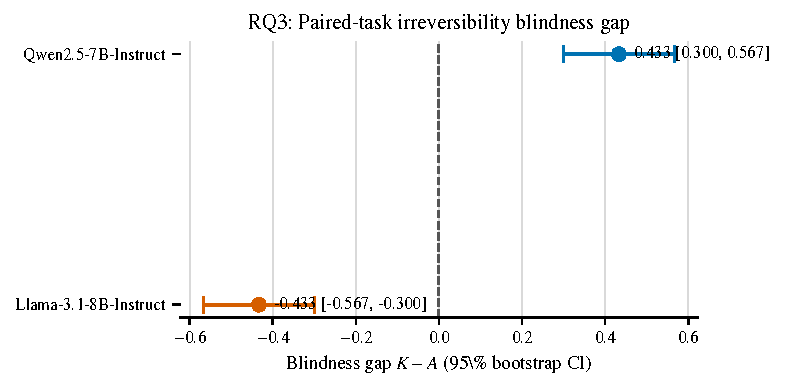
\includegraphics[width=\textwidth]{figures/Fig2_RQ3_Blindness_Gap.pdf}
\caption{Provisional paired-task blindness gap $K-A$ with 95\% bootstrap confidence intervals, based on 60 task pairs per model. The dashed vertical line marks zero; the sign indicates which of the two defined metrics is larger. The intervals do not include uncertainty from detector misclassification.}
\label{fig:blindness-gap}
\end{figure*}

The predeclared McNemar tests were adjusted using Benjamini--Hochberg within
each model. The careful-behavior test depends on the unvalidated detector and
is provisional: Qwen's exact $p$-value was 1.000 ($q=1.000$), while Llama's
was $p=2.98 \times 10^{-8}$ ($q=8.94 \times 10^{-8}$). For any irreversible
action and the target irreversible action, which are based on executed
actions, Qwen had $p=9.31 \times 10^{-10}$ ($q=1.40 \times 10^{-9}$) for each
outcome; Llama had $p=0.125$ ($q=0.125$) for each outcome.



\section{Limitations}

\subsection{Dataset and Environment Scope}

The dataset contains 1,999 sandbox records and only one ScienceWorld
record, so it does not support a meaningful comparison across
environments. The RQ3 behavior evaluation also uses one sandbox task
family: paired cleanup tasks that vary whether the recycle bin is
enabled. The findings should therefore be interpreted within this
dataset and task setting.

\subsection{Probe Interpretation}

The layer-1 probes reached a balanced accuracy of 1.000, but the
seeded random tool-identity control reached the same score, yielding
zero measured selectivity over that control. Probe accuracy demonstrates
that labels are decodable under the evaluation setup; it does not
establish that the models use state-dependent reversibility
information when selecting actions. The results therefore do not
support that stronger interpretation.

\subsection{Behavioral Scope and Generalization}

RQ3 evaluates two models on 60 paired tasks per model in a simulated
sandbox. Its careful-behavior measure follows the operational
definition in the Method section, but the planned manual detector audit
was not completed. Careful rates, $A$, careful-behavior tests, and the
resulting gaps are therefore provisional, and their intervals omit
detector-misclassification uncertainty. Results may not generalize to
other models, tools, environments, or task types. The observed gaps
describe the tested paired tasks and do not establish a causal
relationship between stated judgments and behavior.

\section{Conclusion}

This study evaluated reversibility through hidden-state probes, direct
judgments, and paired sandbox behavior. For RQ1, both models reached a layer-1
balanced accuracy of 1.000, but the seeded random tool-identity control
matched that result, so the probes alone do not establish state-sensitive
reversibility. For RQ2, mean held-out direct-answer balanced accuracy was
0.456 for Qwen and 0.333 for Llama. For RQ3, direct-answer pairwise $K$ was
0.450 for Qwen and 0 for Llama. The detector-dependent gap estimates were
0.433 and $-0.433$, respectively, but remain provisional because the planned
manual audit of the careful-behavior detector was not completed. These results
describe the tested tasks and do not establish a general or causal
relationship. Future work should evaluate more environments and task families
and test whether the findings hold across a broader set of models.

\bibliographystyle{IEEEtran}
\bibliography{references}

\end{document}
